\documentclass[tikz=true]{standalone}
\begin{document}
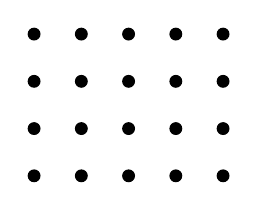
\begin{tikzpicture}
  % Trivial
  \begin{scope}[scale=0.6, every node/.style={draw, shape=circle, fill=black, inner sep=1.5pt, shift={(0,9)}}]
    \node (n00) at (0,0) {};
    \node (n01) at (0,1) {};
    \node (n02) at (0,2) {};
    \node (n03) at (0,3) {};

    \node (n10) at (1,0) {};
    \node (n11) at (1,1) {};
    \node (n12) at (1,2) {};
    \node (n13) at (1,3) {};

    \node (n20) at (2,0) {};
    \node (n21) at (2,1) {};
    \node (n22) at (2,2) {};
    \node (n23) at (2,3) {};

    \node (n30) at (3,0) {};
    \node (n31) at (3,1) {};
    \node (n32) at (3,2) {};
    \node (n33) at (3,3) {};

    \node (n40) at (4,0) {};
    \node (n41) at (4,1) {};
    \node (n42) at (4,2) {};
    \node (n43) at (4,3) {};
  \end{scope}
\end{tikzpicture}
\end{document}
